\documentclass[simplex.tex]{subfiles}
% NO NEED TO INPUT PREAMBLES HERE
% packages are inherited; you can compile this on its own
\subsection{FlashY}
%FlashY is created to encapsulate the R packages created for
%multiple-graph processing and clustering. 
%
%
%When multiple graphs are involved, the dimensionality problem becomes
%more challenging -- since each graph is a matrix, stacking multiple
%graphs leads to a 3-dimensional array referred as tensor. There has been
%little research in handling this type of data in the network data
%domain. A dimension reduction toolbox, to be used in R, has been created
%to convert each adjacency matrix into a small vector, while retaining
%most of the variability across subjects. We tested, as shown in Figure
%\ref{fig:flashy}, the classification performance using sex as outcome
%labels and brain network as input, the low dimensional vector produced
%indistinguishably good performance as the large network data.
%
%
%\begin{figure}[h!]
%\begin{cframed}
%\centering
%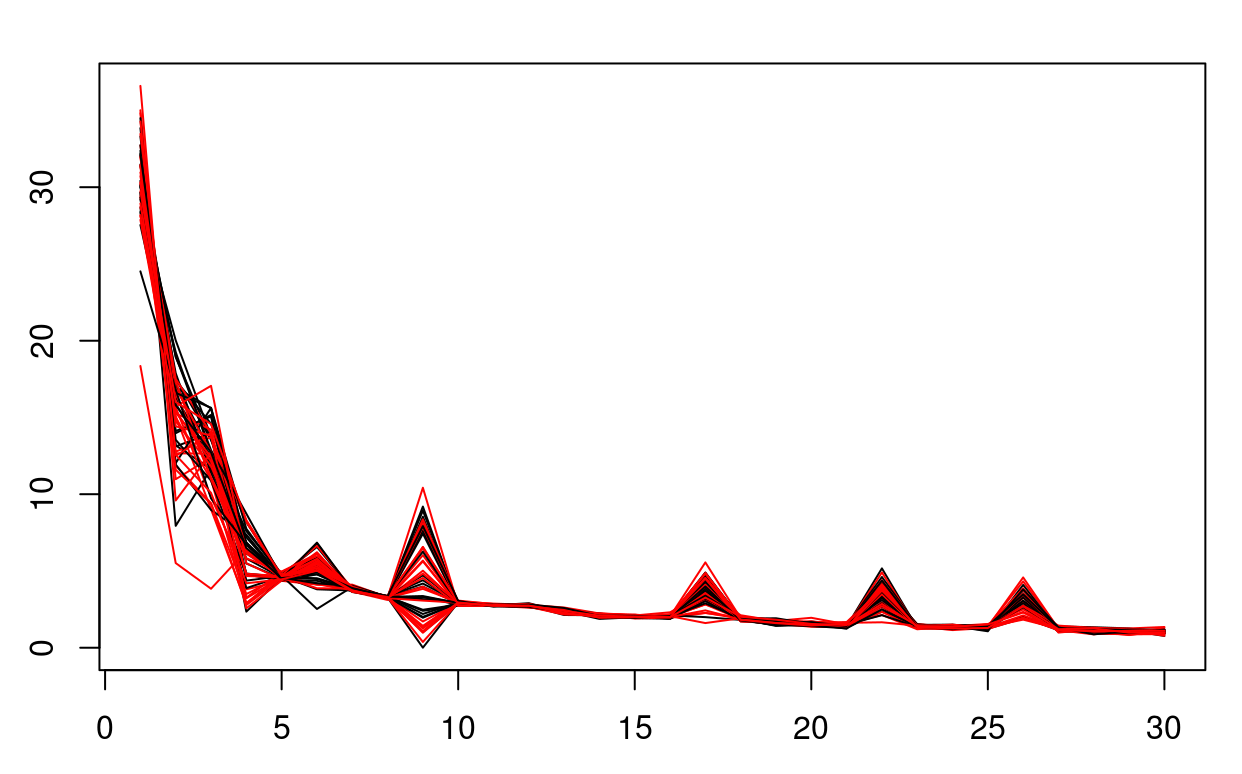
\includegraphics[width=0.75\textwidth]{../../figs/flashY.png}
%\caption{
%View of the low-dimensional vectors from 46 subjects, dimension is
%reduced from 4,900 to only 30 for each subject.
%}
%\label{fig:flashy}
%\end{cframed}
%\end{figure}
%
%We consider improving the stability in clustering objects. When the
%sample size is low but there is large variability due to the high
%dimension, the inferences based on the existing clustering methods
%(k-means, Gaussian mixture model, etc.) tend to produce large error.
%This problem is critical and common in graph clustering, as the number
%of graphs is typically low but the number of vertices is high. To solve
%this, a new clustering method, namely ``jk-means'' is developed in R.
%With a truncation, substantial error reduction can be obtained via the
%bias-variance tradeoff. Shown in the figure, the new jk-means clustering
%tool (red) produces significantly better result than the other models.
%
%
%\begin{figure}[h!]
%\begin{cframed}
%\centering
%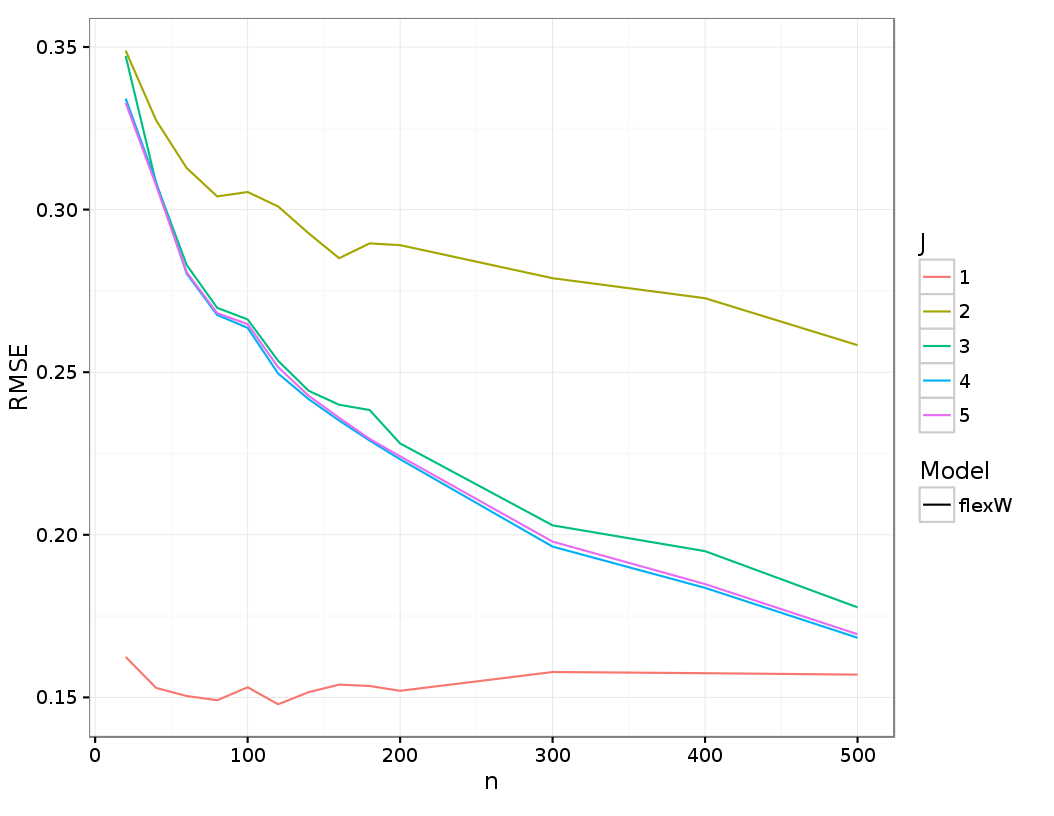
\includegraphics[width=0.75\textwidth]{../../figs/jkmeans.png}
%\caption{
%Illustration of the jk-means, compared with Gaussian Mixture Model (j=5). The j=1 jk-means model (red) has significantly lower error compared to the others, when the sample size is smaller than 500.
%}
%\label{fig:jkmeans}
%\end{cframed}
%\end{figure}
\end{document}
